% F049: native TikZ/PGFPlots, computed from the stated mathematical model.
\begin{center}
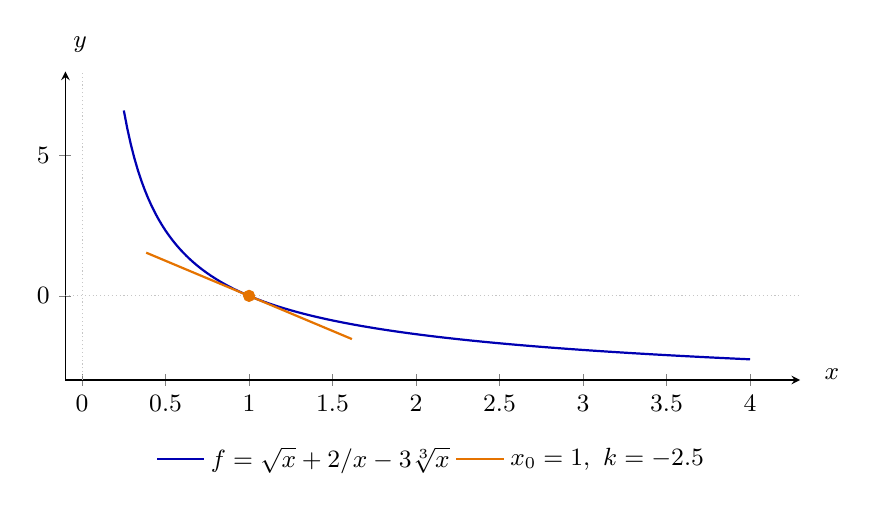
\begin{tikzpicture}[font=\small,>=stealth]
\begin{axis}[width=.90\linewidth,height=5.5cm,xmin=-0.1,xmax=4.3,ymin=-3,ymax=8,
axis lines=left,xlabel={$x$},ylabel={$y$},font=\small,
xlabel style={at={(axis description cs:1.02,.02)},anchor=west},
ylabel style={rotate=-90,at={(axis description cs:.02,1.03)},anchor=south},
legend style={at={(axis description cs:.5,-.18)},anchor=north,draw=none,fill=none,font=\small,legend columns=2},
unbounded coords=jump,clip=true,]
\addplot[gray!45,thin,densely dotted,forget plot] coordinates {(-0.1,0) (4.3,0)};
\addplot[gray!45,thin,densely dotted,forget plot] coordinates {(0,-3) (0,8)};
\addplot[blue!70!black,thick] coordinates {(0.25,6.6101184) (0.27083333,5.9640479) (0.29166667,5.407676) (0.3125,4.9232038) (0.33333333,4.4972664) (0.35416667,4.1196317) (0.375,3.7823314) (0.39583333,3.4790674) (0.41666667,3.2047949) (0.4375,2.9554247) (0.45833333,2.7276071) (0.47916667,2.5185712) (0.5,2.3260052) (0.52083333,2.1479644) (0.54166667,1.9828011) (0.5625,1.8291101) (0.58333333,1.6856851) (0.60416667,1.5514848) (0.625,1.4256055) (0.64583333,1.3072592) (0.66666667,1.1957552) (0.6875,1.0904859) (0.70833333,0.9909142) (0.72916667,0.89656396) (0.75,0.80701118) (0.77083333,0.72187721) (0.79166667,0.64082276) (0.8125,0.56354291) (0.83333333,0.48976284) (0.85416667,0.41923417) (0.875,0.35173186) (0.89583333,0.28705148) (0.91666667,0.22500695) (0.9375,0.16542844) (0.95833333,0.10816068) (0.97916667,0.053061406) (1,0) (1.0208333,-0.051143664) (1.0416667,-0.10048027) (1.0625,-0.14811198) (1.0833333,-0.19413323) (1.1041667,-0.23863147) (1.125,-0.28168779) (1.1458333,-0.3233775) (1.1666667,-0.36377063) (1.1875,-0.40293243) (1.2083333,-0.44092369) (1.2291667,-0.4778012) (1.25,-0.51361805) (1.2708333,-0.5484239) (1.2916667,-0.5822653) (1.3125,-0.61518591) (1.3333333,-0.64722671) (1.3541667,-0.67842624) (1.375,-0.70882074) (1.3958333,-0.73844436) (1.4166667,-0.76732927) (1.4375,-0.79550585) (1.4583333,-0.82300276) (1.4791667,-0.8498471) (1.5,-0.87606452) (1.5208333,-0.90167928) (1.5416667,-0.92671438) (1.5625,-0.95119163) (1.5833333,-0.97513169) (1.6041667,-0.99855424) (1.625,-1.0214779) (1.6458333,-1.0439205) (1.6666667,-1.0658989) (1.6875,-1.0874291) (1.7083333,-1.1085265) (1.7291667,-1.1292057) (1.75,-1.1494806) (1.7708333,-1.1693645) (1.7916667,-1.1888702) (1.8125,-1.2080097) (1.8333333,-1.2267947) (1.8541667,-1.2452363) (1.875,-1.2633451) (1.8958333,-1.2811312) (1.9166667,-1.2986044) (1.9375,-1.3157741) (1.9583333,-1.3326491) (1.9791667,-1.3492382) (2,-1.3655496) (2.0208333,-1.3815911) (2.0416667,-1.3973705) (2.0625,-1.4128949) (2.0833333,-1.4281715) (2.1041667,-1.443207) (2.125,-1.4580079) (2.1458333,-1.4725806) (2.1666667,-1.486931) (2.1875,-1.5010649) (2.2083333,-1.514988) (2.2291667,-1.5287057) (2.25,-1.5422232) (2.2708333,-1.5555455) (2.2916667,-1.5686775) (2.3125,-1.5816239) (2.3333333,-1.5943891) (2.3541667,-1.6069777) (2.375,-1.6193937) (2.3958333,-1.6316414) (2.4166667,-1.6437246) (2.4375,-1.6556471) (2.4583333,-1.6674128) (2.4791667,-1.6790251) (2.5,-1.6904876) (2.5208333,-1.7018036) (2.5416667,-1.7129763) (2.5625,-1.7240089) (2.5833333,-1.7349045) (2.6041667,-1.745666) (2.625,-1.7562963) (2.6458333,-1.7667983) (2.6666667,-1.7771745) (2.6875,-1.7874276) (2.7083333,-1.7975603) (2.7291667,-1.8075749) (2.75,-1.8174739) (2.7708333,-1.8272596) (2.7916667,-1.8369342) (2.8125,-1.8465) (2.8333333,-1.8559592) (2.8541667,-1.8653138) (2.875,-1.8745658) (2.8958333,-1.8837172) (2.9166667,-1.89277) (2.9375,-1.901726) (2.9583333,-1.910587) (2.9791667,-1.9193549) (3,-1.9280312) (3.0208333,-1.9366178) (3.0416667,-1.9451162) (3.0625,-1.9535281) (3.0833333,-1.9618549) (3.1041667,-1.9700983) (3.125,-1.9782597) (3.1458333,-1.9863404) (3.1666667,-1.9943421) (3.1875,-2.0022659) (3.2083333,-2.0101133) (3.2291667,-2.0178855) (3.25,-2.0255838) (3.2708333,-2.0332096) (3.2916667,-2.0407639) (3.3125,-2.0482479) (3.3333333,-2.0556629) (3.3541667,-2.0630099) (3.375,-2.0702901) (3.3958333,-2.0775045) (3.4166667,-2.0846542) (3.4375,-2.0917402) (3.4583333,-2.0987636) (3.4791667,-2.1057253) (3.5,-2.1126262) (3.5208333,-2.1194673) (3.5416667,-2.1262496) (3.5625,-2.1329739) (3.5833333,-2.1396412) (3.6041667,-2.1462522) (3.625,-2.1528078) (3.6458333,-2.1593089) (3.6666667,-2.1657562) (3.6875,-2.1721506) (3.7083333,-2.1784928) (3.7291667,-2.1847836) (3.75,-2.1910238) (3.7708333,-2.1972139) (3.7916667,-2.2033549) (3.8125,-2.2094472) (3.8333333,-2.2154918) (3.8541667,-2.2214891) (3.875,-2.22744) (3.8958333,-2.2333449) (3.9166667,-2.2392046) (3.9375,-2.2450197) (3.9583333,-2.2507908) (3.9791667,-2.2565184) (4,-2.2622032)};
\addlegendentry{$f=\sqrt x+2/x-3\sqrt[3]x$}
\addplot[orange!90!black,thick] coordinates {(0.384,1.54) (1.616,-1.54)};
\addlegendentry{$x_0=1,\ k=-2.5$}
\addplot[only marks,mark=*,orange!90!black,forget plot] coordinates {(1,0)};

\end{axis}
\end{tikzpicture}
\par\smallskip{\small 按本题原函数绘图；切线斜率由本题的导函数计算。}
\end{center}
